\documentclass[tikz]{standalone}

%\input{0-PREAMBULO}


%%-------------------------------------------------------------------------------------
% PREÁMBULO:
%-------------------------------------------------------------------------------------


% MIS PAQUETES
\usepackage{comment}
\usepackage{tikz}
\usepackage{pgfplots}

% MIS COLORES 
\usepackage{xcolor} 
\definecolor{MiAzul}{RGB}{5,108,217} 
\definecolor{MiVerde}{RGB}{43,162,24}
\definecolor{MiLila}{RGB}{180,127,252} 
\definecolor{NaranjaCruzzi}{RGB}{227,132,27}
%\definecolor{MiDodgerBlue}{RGB}{47,169,250}
%\definecolor{MiNaranja}{RGB}{207,110,46}
%\definecolor{NaranjaPokemonOro}{RGB}{242,92,39}

% CAP 1
\usetikzlibrary{
   arrows.meta,
  intersections,
}

% CAP 2
\pgfplotsset{compat=newest}
\pgfplotsset{soldot/.style={color=MiAzul,only marks,mark=*}} \pgfplotsset{holdot/.style={color=MiAzul,fill=white,only marks,mark=*}}


%-------------------------------------------------------------------------------------
%FIN PREÁMBULO
%-------------------------------------------------------------------------------------


\begin{document}

%-------------------------------------------------------------------------------------
%------------------------------------- CAP 1 -----------------------------------------
%-------------------------------------------------------------------------------------

% FIGURA 1.1: Funcion convexa.
% Requiere reconfigurar ejes.

{\pgfplotsset{plot coordinates/math parser=false} 
\pgfplotsset{
    every non boxed x axis/.style={
        xtick align=center,
        enlarge x limits=true,
        x axis line style={line width=0.8pt, -latex}
},
    every boxed x axis/.style={}, enlargelimits=false
}
\pgfplotsset{
    every non boxed y axis/.style={
        ytick align=center,
        enlarge y limits=true,
        y axis line style={line width=0.8pt, -latex}
},
    every boxed y axis/.style={}, enlargelimits=false
}

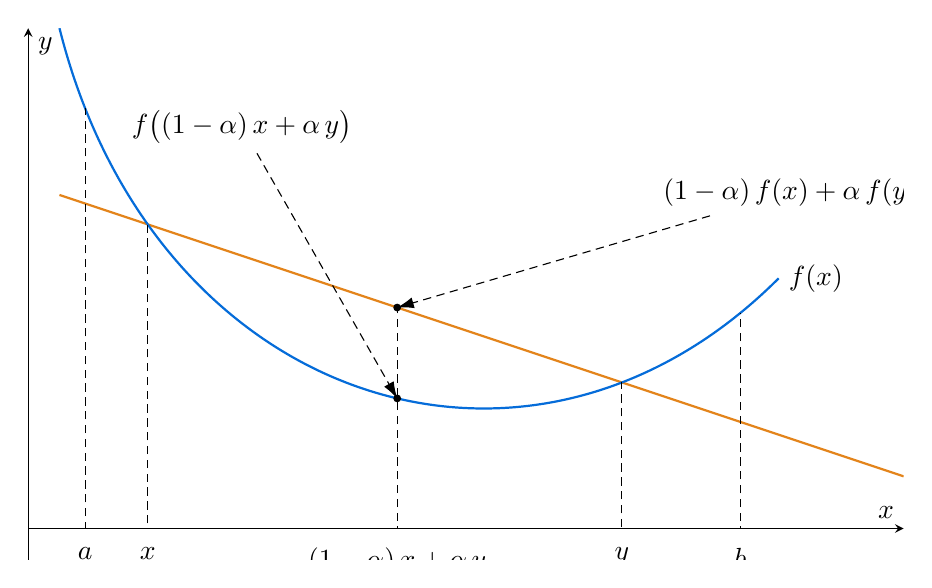
\begin{tikzpicture}
\begin{axis}[
    %width=1\textwidth,
    %height=0.8\textwidth,
    width=5in, axis equal image,
    axis lines=middle,
    xmin=0,xmax=7,
    xlabel=$x$,ylabel=$y$,
    ymin=-0.25,ymax=4,
    xtick={\empty},ytick={\empty}, axis on top
]


\addplot[thick,domain=0.25:7,NaranjaCruzzi,name path = A]  {-x/3 + 2.75} coordinate[pos=0.4] (m) ;
\draw[thick,MiAzul, name path =B] (0.25,4) .. controls (1,1) and (4,0) .. (6,2) node[pos=1.00, color=black, right]  {$f(x)$} coordinate[pos=0.075] (a1)  coordinate[pos=0.95] (a2);
\path [name intersections={of=A and B, by={a,b}}];


\draw[densely dashed] (0,0) -| node[pos=0.5, color=black, label=below:$a$] {}(a1);
\draw[densely dashed] (0,0) -| node[pos=0.5, color=black, label=below:$x$] {}(a);
\draw[densely dashed, name path=D] (3,0) -|node[pos=0.5, color=black, label=below: $\left( 1 - \alpha \right) x + \alpha \, y $] {} node[pos=1, fill,circle,inner sep=1pt] {}(m);
\draw[densely dashed] (0,0) -|node[pos=0.5, color=black, label=below:$y$] {}(b);
\draw[densely dashed] (0,0) -|node[pos=0.5, color=black, label=below:$b$] {}(a2);


\path [name intersections={of=B and D, by={c}}] node[fill,circle,inner sep=1pt] at (c) {}; 


\node[anchor=south west, text=black] (d) at (0.75,3) {$f \bigl( \left( 1 - \alpha \right) x + \alpha \, y \bigr)$};
\node[anchor=south west, text=black] (e) at (5,2.5) {$\left( 1 - \alpha \right) f(x) + \alpha \, f(y)$};
\draw[-{Latex[width=4pt,length=6pt]}, densely dashed] (d) -- (c);
\draw[-{Latex[width=4pt,length=6pt]}, densely dashed] (e) -- (m);
\end{axis}
\end{tikzpicture}

}

%-------------------------------------------------------------------------------------

% FIGURA 1.2: Funcion convexa. Bis.

{\pgfplotsset{plot coordinates/math parser=false} 
\pgfplotsset{
    every non boxed x axis/.style={
        xtick align=center,
        enlarge x limits=true,
        x axis line style={line width=0.8pt, -latex}
},
    every boxed x axis/.style={}, enlargelimits=false
}
\pgfplotsset{
    every non boxed y axis/.style={
        ytick align=center,
        enlarge y limits=true,
        y axis line style={line width=0.8pt, -latex}
},
    every boxed y axis/.style={}, enlargelimits=false
}

\begin{tikzpicture}
\begin{axis}[
    %width=1\textwidth,
    %height=0.8\textwidth,
    width=5in, axis equal image,
    axis lines=middle,
    xmin=0,xmax=9,
    xlabel=$x$,ylabel=$y$,
    ymin=-0.25,ymax=8,
    xtick={\empty},ytick={\empty}, axis on top
]

\addplot[thick,domain=0.9:3.2,NaranjaCruzzi,name path = A]  {-x/4 + 2.75} coordinate[pos=0.4] (m) ;
\draw[thick,MiAzul, name path =B] (0.25,4) .. controls (1,1) and (4,0) .. (8,8) node[pos=1.00, color=black, right]  {$f(x)$} coordinate[pos=0.075] (a1)  coordinate[pos=0.95] (a2);
\path [name intersections={of=A and B, by={a,b}}];


\draw[densely dashed] (0,0) -| node[pos=0.5, color=black, label=below:$x$] {}(a);

\draw[densely dashed] (0,0) -|node[pos=0.5, color=black, label=below:$y$] {}(b);
\draw[densely dashed] (0,0) -|node[pos=0.5, color=black,fill,circle,inner sep=1pt, label=below:$z$] {}(6.4,5.2);

% PRIMERO: Dibujo líneas.

\draw [thick,MiVerde] (a) -- (6.4,5.2);
\draw [thick,MiLila] (b) -- (6.4,5.2);

% DESPUÉS: Dibujo puntos.

\path node[fill,circle,inner sep=1pt, in front of path,] at (a) {}; 
\path [name intersections={of=B and D, by={c}}] node[fill,circle,inner sep=1pt] at (b) {}; 
\path node[fill,circle,inner sep=1pt] at (6.4,5.2) {}; 
\end{axis}
\end{tikzpicture}

}

%-------------------------------------------------------------------------------------

% FIGURA 1.3: Funcion convexa. Mínimo.

\begin{tikzpicture}[scale=1]
        \begin{axis}[
        width=1\textwidth,
        height=1\textwidth,
        xmin = -0.5, xmax = 6.1, 
        ymin = -0.5, ymax = 5,  
        restrict y to domain=-1:30,
        axis lines = middle,
        axis line style={-latex},  
        xlabel={$x$},
        ylabel={},
        %enlarge x limits={upper={val=0.2}},
        enlarge y limits=0.05,
        x label style={at={(ticklabel* cs:1.00)}, inner sep=5pt, anchor=north},
        y label style={at={(ticklabel* cs:1.00)}, inner sep=5pt, anchor=south east},
        xtick = {-2,-1,0,1,2,3,4,5},
        ytick = {1,2,3,4},
        xticklabels = {$-2$,$-1$,$0$,$1$,$2$,$3$,$4$,$5$}, %INTERPOLA !
        yticklabels = {$1$,$2$,$3$,$4$},
        ]

        \addplot[domain=0:1,MiAzul, smooth, thick] {1/x};  
        \addplot[domain=1:2,MiAzul, smooth, thick] {1};
        \addplot[domain=2:6,MiAzul, smooth, thick] {x-1} node[black,midway,left,pos=0.5] {$f(x)$};

        % PUNTOS DE DISCONTINUIDAD: 
        % soldot -> solidos (rellenos). holdot -> vacíos
        %\addplot[holdot] coordinates{(0,0)(1,0)(2,0)(3,0)(4,0)(5,0)};
        \addplot[soldot] coordinates{(1,1)(2,1)};%(3,2)(4,6)(5,24)};

        \end{axis}
\end{tikzpicture}

%-------------------------------------------------------------------------------------

% FIGURA 1.4: Funcion convexa. Mínimo. Bis.

\begin{tikzpicture}[scale=1]
        \begin{axis}[
        width=1\textwidth,
        height=1\textwidth,
        xmin = -3.1, xmax = 3.1, 
        ymin = -0.5, ymax = 10,  
        restrict y to domain=-1:30,
        axis lines = middle,
        axis line style={-latex},  
        xlabel={$x$},         
        ylabel={},
        %enlarge x limits={upper={val=0.2}},
        enlarge y limits=0.05,
        x label style={at={(ticklabel* cs:1.00)}, inner sep=5pt, anchor=north},
        y label style={at={(ticklabel* cs:1.00)}, inner sep=5pt, anchor=south east},
        xtick = {-3,-2,-1,0,1,2,3},
        ytick = {1,4,9},
        xticklabels = {$-3$,$-2$,$-1$,$0$,$1$,$2$,$3$}, %INTERPOLA !
        yticklabels = {$1$,$4$,$9$},
        ]

        \addplot[domain=-4:4,MiAzul, smooth, thick] {x*x} node[black,midway,left,pos=0.65] {$f(x) = x^2$}; 
        \addplot[soldot] coordinates{(0,0)};

        \end{axis}
\end{tikzpicture}


%-------------------------------------------------------------------------------------
%------------------------------------- CAP 2 -----------------------------------------
%-------------------------------------------------------------------------------------


% FIGURA 2.1: Gamma real.

\begin{tikzpicture}[scale=1]
        \begin{axis}[
        width=1\textwidth,
        height=1\textwidth,
        xmin = -4.9, xmax = 6.1, 
        %ymin = -3.5, ymax = 3.5,  
        restrict y to domain=-10:25,
        axis lines = middle,
        axis line style={-latex},  
        xlabel={$x$}, 
        ylabel={$\Gamma{(x)}$},
        %enlarge x limits={upper={val=0.2}},
        enlarge y limits=0.05,
        x label style={at={(ticklabel* cs:1.00)}, inner sep=5pt, anchor=north},
        y label style={at={(ticklabel* cs:1.00)}, inner sep=5pt, anchor=south east},
        xtick = {-4,-3,-2,-1,0,1,2,3,4,5},
        ytick = {2,6,24},
        xticklabels = {$-4$,$-3$,$-2$,$-1$,$0$,$1$,$2$,$3$,$4$,$5$}, 
        yticklabels = {$2$,$6$,$24$},
        ]
        % Gamma para x > 0
        \addplot[color=MiAzul, samples=1200, smooth, thick,
        domain = 0:6] gnuplot{gamma(x)};

        % Gamma para x < 0
        \foreach[evaluate={\N=\n-1}] \n in {0,...,-5}{%
        \addplot[color=MiAzul, samples=555, smooth, thick, 
        domain = \n:\N] gnuplot{gamma(x)};
        
        % Asíntotas
        \addplot [domain=-20:30, samples=200, densely dotted, thin] (\N, x);
        }
        
        % Puntos (x,Gamma(x)), x = 1,...,5. Gamma(n)=(n-1)!

        \addplot+[only marks, color=NaranjaCruzzi, mark=*] coordinates {(1,1) (2,1) (3,2) (4,6) (5,24)};
        
        \end{axis}
\end{tikzpicture}

%-------------------------------------------------------------------------------------

% FIGURA 2.2: Pseudogamma. Caso degenerado.

\begin{tikzpicture}[scale=1]
        \begin{axis}[
        width=1\textwidth,
        height=1\textwidth,
        xmin = -0.5, xmax = 6.1, 
        ymin = -0.5, ymax = 25,  
        restrict y to domain=-1:30,
        axis lines = middle,
        axis line style={-latex},  
        xlabel={$y$},         %En esta parte del trabajo llamo `y' a la variable real
        ylabel={$f{(y)}$},
        %enlarge x limits={upper={val=0.2}},
        enlarge y limits=0.05,
        x label style={at={(ticklabel* cs:1.00)}, inner sep=5pt, anchor=north},
        y label style={at={(ticklabel* cs:1.00)}, inner sep=5pt, anchor=south east},
        xtick = {-2,-1,0,1,2,3,4,5},
        ytick = {1,2,6,24},
        xticklabels = {$-2$,$-1$,$0$,$1$,$2$,$3$,$4$,$5$}, %INTERPOLA !
        yticklabels = {$1$,$2$,$6$,$24$},
        ]

        % f IDENTICAMENTE NULA
        \addplot[domain=0:1,MiAzul, smooth, thick] {0};
        \addplot[domain=1:2,MiAzul, smooth, thick] {0};
        \addplot[domain=2:3,MiAzul, smooth, thick] {0};
        \addplot[domain=3:4,MiAzul, smooth, thick] {0};
        \addplot[domain=4:5,MiAzul, smooth, thick] {0};
        \addplot[domain=5:6,MiAzul, smooth, thick] {0};

        % LINEAS VERTICALES PUNTEADAS
        \draw[dotted] (axis cs:1,0) -- (axis cs:1,1);
        \draw[dotted] (axis cs:2,0) -- (axis cs:2,1);
        \draw[dotted] (axis cs:3,0) -- (axis cs:3,2);
        \draw[dotted] (axis cs:4,0) -- (axis cs:4,6);
        \draw[dotted] (axis cs:5,0) -- (axis cs:5,24);
        
        % PUNTOS DE DISCONTINUIDAD: soldot -> solidos (rellenos). holdot -> vacíos
        \addplot[holdot] coordinates{(0,0)(1,0)(2,0)(3,0)(4,0)(5,0)};
        \addplot[soldot] coordinates{(1,1)(2,1)(3,2)(4,6)(5,24)};

        \end{axis}
\end{tikzpicture}

%-------------------------------------------------------------------------------------

% FIGURA 2.3: Pseudogamma. Caso continuo.

\begin{tikzpicture}[scale=1]
        \begin{axis}[
        width=1\textwidth,
        height=1\textwidth,
        xmin = -0.5, xmax = 6.1, 
        ymin = -0.5, ymax = 25,  
        restrict y to domain=-1:30,
        axis lines = middle,
        axis line style={-latex},  
        xlabel={$y$},         %En esta parte del trabajo llamo `y' a la variable real
        ylabel={$f{(y)}$},
        %enlarge x limits={upper={val=0.2}},
        enlarge y limits=0.05,
        x label style={at={(ticklabel* cs:1.00)}, inner sep=5pt, anchor=north},
        y label style={at={(ticklabel* cs:1.00)}, inner sep=5pt, anchor=south east},
        xtick = {-2,-1,0,1,2,3,4,5},
        ytick = {1,2,6,24},
        xticklabels = {$-2$,$-1$,$0$,$1$,$2$,$3$,$4$,$5$}, %INTERPOLA !
        yticklabels = {$1$,$2$,$6$,$24$},
        ]
 
        \addplot[domain=0:1,MiAzul, smooth, thick] {1/x};
        \addplot[domain=1:2,MiAzul, smooth, thick] {1};
        \addplot[domain=2:3,MiAzul, smooth, thick] {x-1};
        \addplot[domain=3:4,MiAzul, smooth, thick] {(x-2)*(x-1)};
        \addplot[domain=4:5,MiAzul, smooth, thick] {(x-3)*(x-2)*(x-1)};
        \addplot[domain=5:6,MiAzul, smooth, thick] {(x-4)*(x-3)*(x-2)*(x-1)};
        %\addplot[domain=5:6,MiAzul, smooth, thick] {0};

        %LINEAS VERTICALES PUNTEADAS
        \draw[dotted] (axis cs:1,0) -- (axis cs:1,1);
        \draw[dotted] (axis cs:2,0) -- (axis cs:2,1);
        \draw[dotted] (axis cs:3,0) -- (axis cs:3,2);
        \draw[dotted] (axis cs:4,0) -- (axis cs:4,6);
        \draw[dotted] (axis cs:5,0) -- (axis cs:5,24);
        
        %PUNTOS DE DISCONTINUIDAD: soldot -> solidos (rellenos). holdot -> vacíos
        %\addplot[holdot] coordinates{(0,0)(1,0)(2,0)(3,0)(4,0)(5,0)};
        \addplot[soldot] coordinates{(1,1)(2,1)(3,2)(4,6)(5,24)};

        \end{axis}
\end{tikzpicture}

%-------------------------------------------------------------------------------------

% FIGURA 2.4: Gamma real. Zoom en [1,2].

\begin{tikzpicture}[scale=1]
        \begin{axis}[
        width=1\textwidth,
        height=1\textwidth,
        xmin = 0.9, xmax = 2.1 , 
        %ymin = -3.5, ymax = 3.5,  
        restrict y to domain=-1:5
        axis lines = center,
        axis line style={-latex},  
        xlabel={$x$}, 
        ylabel={$\Gamma{(x)}$},
        enlarge x limits={upper={val=0.2}},
        enlarge y limits=0.05,
        x label style={at={(ticklabel* cs:1.00)}, inner sep=5pt, anchor=north},
        y label style={at={(ticklabel* cs:1.00)}, inner sep=5pt, anchor=south east},
        xtick = {0,1,1.5,2},
        ytick = {0,1},
        xticklabels = {$0$,$1$,$1.5$,$2$}, %INTERPOLA !
        yticklabels = {$0$,$1$},
        ]
        
        \addplot[color=MiAzul, samples=200, smooth, thick,
        domain = 0.9:2.2] gnuplot{gamma(x)};
        
        \addplot[color=NaranjaCruzzi, mark=*] coordinates {(1,1)};
        \addplot[color=NaranjaCruzzi, mark=*] coordinates {(2,1)};     
        \end{axis}
\end{tikzpicture}







\end{document}
